\chapter{Discussion}
Please tell more about conclusion and how to the next work of this study.

\section{Cokro Edi Prawiro / 1164069}
\subsection{Teori}

\begin{enumerate}

\item Jelaskan Kenapa file teks harus dilakukan tokenizer. Dilengkap dengan ilustrasi atau gambar.\par
Tokenizer adalah proses untuk membagi kalimat menjadi beberapa teks, hal ini sangat di perlukan dalam AI karena nanti setiap teks akan di hitung bobotnya dang akan memunculkan nilai vektor sehingga teks tersebut bisa di gunakan sebagai data untuk memprediksi teks yang muncul dalam satu kalimat sedangakan proses tkenizer merupakan caramembagi bagi teks dari suatu kalimat biasanya pembagi kalimat tersebut merupakan spasi dalan suatu kalimat. Agar lebih jelas dapat melihat gamabr \ref{c131} berikut. 

\begin{figure}[!htbp]
      \centering{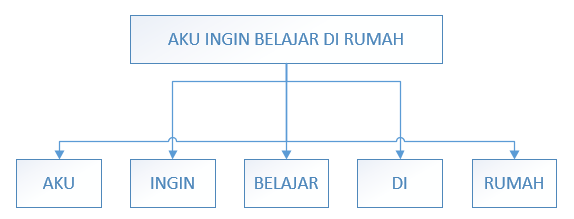
\includegraphics[width=0.7\textwidth]
      {figures/cokro/c131}}
      \caption{Ilustrasi Tokenisasi}
      \label{c131}
      \end{figure}

\item jelaskan konsep dasar K Fold Cross VAlidation dan dataset komentar youtube pada code berikut dilengkapi dengan ilustrasi gambar  
\begin{verbatim}
kfold = StartifiedKFlod(n_splits=5)
splits = kfold.split(d, d['CLASS'])
\end{verbatim}
pada codingan tersebut terdapat kfold sebagai variabel yang didalammnya terdiri dari split 5 yang berarti pengulangan terhadap pengolahan masing masing lima kali pada kasus ini terdapat data sebanyak 5 berarti ke lima data tersebut di ulang sebanyak lima kali dengan atribut class sebagai acuan pengolahan datanya kemudian akan di hasilkan akurasi dari pengulangan data tersebut sebesar sekian persen tergantung datanya. agar lebih jelas dapat di lihat pada gambar \ref{c132}  berikut:

\begin{figure}[!htbp]
      \centering{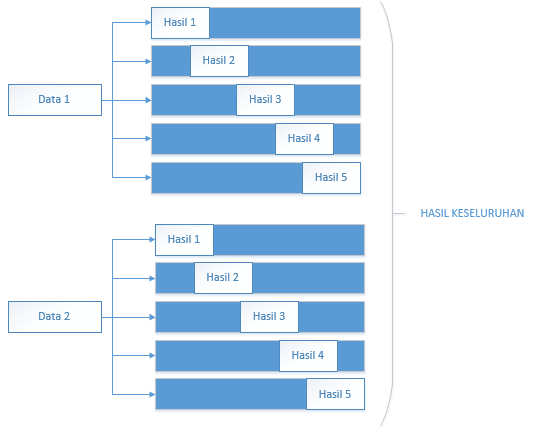
\includegraphics[width=0.7\textwidth]
      {figures/cokro/c132}}
      \caption{Ilustrasi K Fold Cross Validation}
      \label{c132}
      \end{figure}

\item Jelaskan apa maksudnya kode program for train, test in split dilengkapi di lengkapi dengan ilustrasi atau gambar.\par
for train di gunakan melakukan training atau pelatihan terhadap data yang telah di deklarasikan sebelumnya. sedangkan test in split di gunakan untuk diguanakan untuk membatasi jumlah data yang akan di inputkan atau data yang akan di gunakan.agar lebih jelas dapat di lihat pada gambar \ref{c133} berikut.

\begin{figure}[!htbp]
      \centering{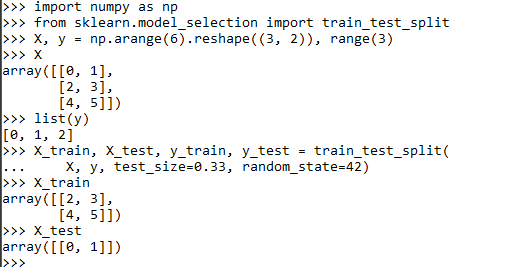
\includegraphics[width=0.7\textwidth]
      {figures/cokro/c133}}
      \caption{Ilustrasi For Train dan Test in split}
      \label{c133}
      \end{figure}

\item Jelaskan apa maksud kode program traint\_content =d['CONTENT'].iloc[traint\_idx] dan test\_content =d['CONTENT'].iloc[traint\_idx]. dilengkapi dengan ilustrasi atau gambar.\par
maksud dari kode program tersebut adalah membaca isian kolom pada field yang bernama CONTENT sebagai data training dan data testing untuk program tersebut sebagai ilustrasi dapat di lihat pada gambar \ref{c134} berikut.

\begin{figure}[!htbp]
      \centering{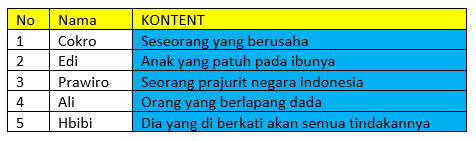
\includegraphics[width=0.7\textwidth]
      {figures/cokro/c134}}
      \caption{Ilustrasi Penggunaan kolom CONTENT}
      \label{c134}
      \end{figure}

\item Jelaskan maksud dari fungsi tokenizer = Tokennizer(num\_words=2000)dan tokenizer.fit\_on\_texts(train\_konten) di lengkapi dengan ilustrasi gambar.\par
fungsi tokenizer = Tokennizer(num\_words=2000) digunakan untuk membaca kalimat yang telah di buat menjadi token sebanyak 2000 kata dan fingsi fit\_on\_texts(train\_konten) digunakan untuk membuat membaca data token teks yang telah di masukan kedalam fungsi yaitu fungsi train\_konten. agar lebih jelas dapat di lihat pada gambar \ref{c135} berikut.

\begin{figure}[!htbp]
      \centering{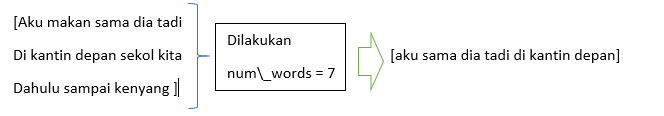
\includegraphics[width=0.7\textwidth]
      {figures/cokro/c135}}
      \caption{Ilustrasi fit tokenizer dan num\_word=2000}
      \label{c135}
      \end{figure}

\item Jelaskan apa maksud dari fungsi d train inputs = tokenizer.texts to matrix(train content, mode=tfidf) dan d test inputs = tokenizer.texts to matrix(test content, mode=tfidf), dilengkapi dengan ilustrasi kode dan atau gambar.\par 
yaitu di gunakan untuk mengubah urutan teks yang tadi telah di lakukan tokenizer menjadi matriks yang berut=rutan seperti tf idf 
contoh seperti gambar \ref{c136} berikut.

\begin{figure}[!htbp]
      \centering{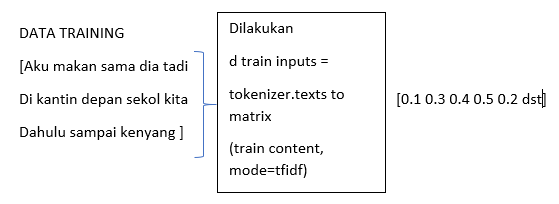
\includegraphics[width=0.7\textwidth]
      {figures/cokro/c136}}
      \caption{Ilustrasi d train inputs = tokenizer.texts to matrix(train content, mode=tfidf)}
      \label{c136}
      \end{figure}

\item Jelaskan apa maksud dari fungsi \emph{d\_train\_inputs = d\_train\_inputs/np.amax(np.absolute(d\_train\_inputs))} dan \emph{d\_test\_inputs = d\_test\_inputs/np.amax(np.absolute(d\_test\_inputs))}, dilengkapi dengan ilustrasi atau gambar \par

fungsi tersebut digunakan untuk membagi matriks tfidf dengan dengan penentuan maksimum aray sepanjang sumbu sehingga akan menimbulkan garis ke bawah dan keatas yang membentuk gambar v kemudian hasil tersebut akan di masukan ke dalam variabel d train input dan d test input dengan methode absolute. yang berarti tanpa bilangan negatif. untuk lebih jelasnya dapat di lihat pada gambar \ref{c137}  berikut ini.

\begin{figure}[!htbp]
      \centering{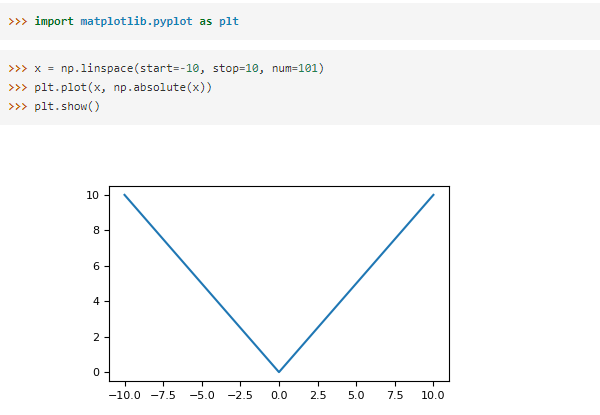
\includegraphics[width=0.7\textwidth]
      {figures/cokro/c137}}
      \caption{Ilustrasi d\_train\_inputs = d\_train\_inputs/np.amax(np.absolute(d\_train\_inputs))}
      \label{c137}
      \end{figure}

\item Jelaskan apa maksud fungsi dari d train outputs = np utils.to categorical(d['CLASS'].iloc[train dan d test outputs = np utils.to categorical(d['CLASS'].iloc[test idx]) dalam kode program, dilengkapi dengan ilustrasi atau gambar.\par

maksud dari fungsi tersebut yaitu untuk merubah nilai vektor yang ada pada atribut class menjadi bentuk matrix dengan pengurutan berdasarkan data index training dan testing. Sebagai contoh dapat di lihat ilustrasi pada gambar \ref{c138} berikut ini.

\begin{figure}[!htbp]
      \centering{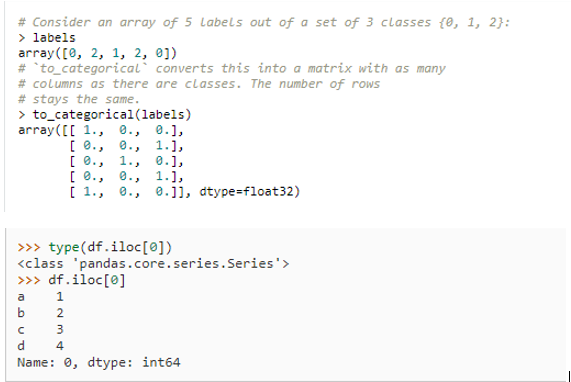
\includegraphics[width=0.7\textwidth]
      {figures/cokro/c138}}
      \caption{Ilustrasid train outputs = np utils.to categorical(d['CLASS'].iloc[train}
      \label{c138}
      \end{figure}

\item Jelaskan Maksud Dari fungsi

\item Jelaskan Maksud Dari Fungsi

\item Jelaskan apa itu Deep Learning \par
merupakan salah satu algoritma jaringan saraf tiruan yang menggunakan meta data sebagai inputan dan mengolahnya menggunakan layer layer yang tersembunyi. deep lerning memiliki suatu keunikan yaitu fitur yang dapat mengekstraksi secara otomatis.

\item Jelaskan Apa itu Deep Neural Network dan apa perbedaanya dengan Deep Learning.\par
merupakan algoritma jaringan syaraf juga yang mena akan melakukan pembobotan terhadap data yang sudah ada sebagai acuan untuk data inputan selanjutnya. kemudian terdiri atas beberapa layer atau hiden layer. perbedaan antara deep learning dan DNN atau Deep Neural Network yaitu deep lerning merupakan pemakai algoritma dari DNN dan DNN merupakan algoritma yang ada pada deep learning.

\item Konfolusi


\end{enumerate}